\documentclass[10pt, aspectratio=169]{beamer}

% Theme Configuration for Professional Look
\usetheme{Madrid}
\usecolortheme{dolphin}
\usefonttheme{professionalfonts}

% Bibliography Setup (APA Style)
\usepackage[style=apa, backend=biber]{biblatex}
\addbibresource{references.bib}

% Title Information
\title[Short Title]{Predictive Biomarkers in Heart Failure: \\ A Logistic Regression Approach}
\subtitle{Master of Science Thesis Defense}
\author{Candidate Name}
\institute[University Abbreviation]{
	Department of Biostatistics \\
	\textbf{Rigor Scientific Solutions} (Analysis \& Formatting Support) \\
	\vspace{0.2cm}
	\textit{Date: \today}
}

\begin{document}
	
	% Slide 1: Title
	\begin{frame}
		\titlepage
	\end{frame}
	
	% Slide 2: Methodology
	\begin{frame}{Methodological Framework}
		\begin{itemize}
			\item \textbf{Objective:} Evaluate predictors of mortality using clinical records.
			\item \textbf{Model:} Binary Logistic Regression with stratified train-test split.
			\item \textbf{Equation:}
			\begin{equation}
				\ln\left(\frac{p}{1-p}\right) = \beta_0 + \beta_1 X_{EF} + \beta_2 X_{Cr} + \epsilon
			\end{equation}
			\item \textbf{Significance:} Model achieved an ROC-AUC of 0.862.
		\end{itemize}
	\end{frame}
	
	% Slide 3: Results Visualization
	\begin{frame}{Key Findings}
		\begin{figure}
			\centering
			% In a real project, you would include the image generated in Sample 3
			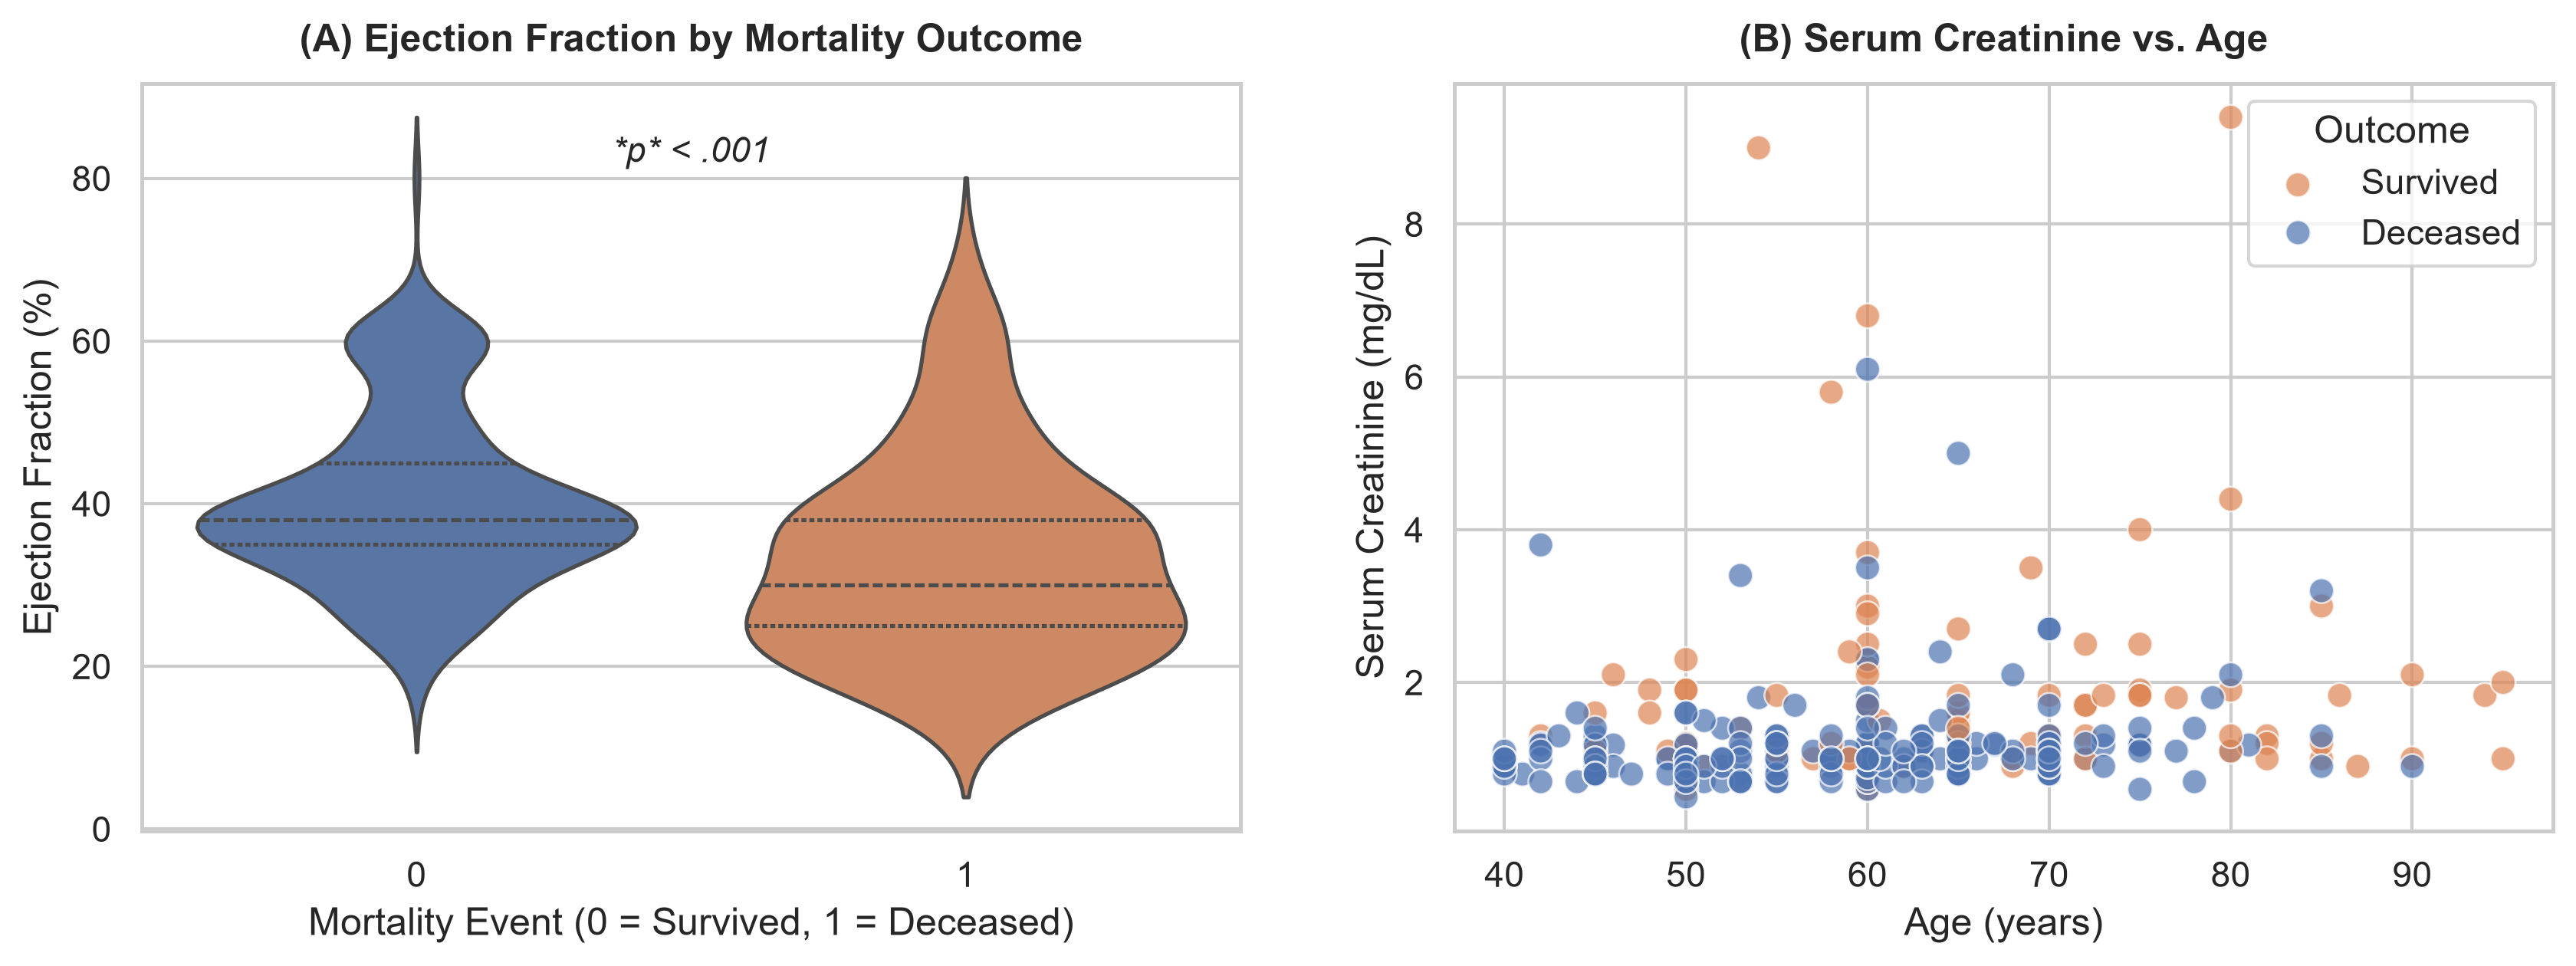
\includegraphics[width=0.8\textwidth]{rigor_scientific_figure_1.png}
			\caption{Distribution of Ejection Fraction and Serum Creatinine by outcome.}
		\end{figure}
	\end{frame}
	
	% Slide 4: References
	\begin{frame}[allowframebreaks]{References}
		\printbibliography[heading=none]
	\end{frame}
	
\end{document}